\documentclass[a4paper,10pt]{article}
\usepackage[utf8]{inputenc}

\usepackage[english]{babel}
\usepackage[dvinames]{xcolor}
\usepackage[compact,small]{titlesec}
\usepackage{booktabs}
\usepackage{multirow}
\usepackage{amsfonts,amsmath,amssymb}
\usepackage{marginnote}
\usepackage[top=1.8cm, bottom=1.8cm, outer=1.8cm, inner=1.8cm, heightrounded, marginparwidth=2.5cm, marginparsep=0.5cm]{geometry}
\usepackage{enumitem}
\setlist{noitemsep,parsep=2pt}
\newcommand{\highlight}[1]{\textcolor{kuleuven}{#1}}
\usepackage{pythonhighlight}
\usepackage{cleveref}
\usepackage{graphicx}

\usepackage{float}
\usepackage{subcaption}
\usepackage{siunitx}

\newcommand{\nextyear}{\advance\year by 1 \the\year\advance\year by -1}
\newcommand{\thisyear}{\the\year}
\newcommand{\deadlineGroup}{November 27, \thisyear{} at 16:00 CET}
\newcommand{\deadlineCode}{December 18, \thisyear{} at 16:00 CET}
\newcommand{\deadlineReport}{January 4, \nextyear{} at 16:00 CET}

\newcommand{\ReplaceMe}[1]{{\color{blue}#1}}
\newcommand{\RemoveMe}[1]{{\color{purple}#1}}

\setlength{\parskip}{5pt}



%opening
\title{Evolutionary Algorithms: Final report}
\author{Simon Perneel}

\begin{document}
\fontfamily{ppl}
\selectfont{}
\setlength\parindent{0pt} % no indentation

\maketitle

% \section{\RemoveMe{Formal requirements}} \label{sec_this}

% \RemoveMe{The report is structured for fair and efficient grading of over 100 individual projects in the space of only a few days. Please respect the exact structure of this document. You are allowed to remove sections \ref{sec_this} and \ref{sec_other}. Brevity is the soul of wit: a good report will be \textbf{around $7$ pages} long. The hard limit is 10 pages. 

% It is recommended that you use this \LaTeX{} template, but you are allowed to reproduce it with the same structure in a WYSIWYG-editor. The purple text containing our evaluation criteria can be removed. You should replace the blue text with your discussion. \textbf{The questions we ask in blue are there to guide which topics to discuss}, rather than an exact list of questions that must be answered. Feel free to add more items to discuss.

% This report should be uploaded to Toledo by \deadlineReport. It must be in the \textbf{Portable Document Format} (pdf) and must be named \texttt{r0123456\_final.pdf}, where r0123456 should be replaced with your student number.}

\section{Metadata}

\begin{itemize}
 \item \textbf{Group members during group phase:} Thomas Feys \& Timo Martens
 \item \textbf{Time spent on group phase:} 12.5 hours
 \item \textbf{Time spent on final code:} 40 hours
 \item \textbf{Time spent on final report:} %todo
\end{itemize}

\section{Modifications since the group phase}

% \RemoveMe{\textbf{Goal:} Based on this section, we will evaluate insofar as you are able to analyse common problems arising in the design and implementation of evolutionary algorithms and your ability to effectively solve them.}

\subsection{Main improvements}

% \ReplaceMe{List the main changes that you implemented since the group phase. You do not need to explain the employed techniques in detail; for this, you should refer to the appropriate subsection of section 3 of the report.}
The following paragraphs briefly describe the main improvements since the group phase. A more detailed explanation is given in section~\ref{sec:design}.

% \paragraph{Short description 1:} \ReplaceMe{State what modification you made (e.g., replaced top-$\lambda$ selection with $k$-tournament selection). What aspect of your evolutionary algorithm did it improve?} 

\paragraph{Initialization of the population:} The population is initialized now with an amount of heuristic good individuals. It leads the search into more promising areas of the search space and speeds up the optimization process. See section~\ref{ssec:initialization}~and~\ref{ssec:localsearch}.
\paragraph{More and better mutation operators:} In addition to swap mutation, insert mutation, scramble mutation and reverse sequence mutation have been implemented in order to increase randomness in the search. It results in more diversity in the population. See section~\ref{ssec:mutation}.
\paragraph{Dpx crossover and cycle crossover:} In addition the order mutation, distance preserving crossover and cycle crossover have been implemented in order to generate more diverse individuals. See section~\ref{ssec:recombination}
\paragraph{Crowding:} The ($\lambda$+$\mu$)-elimination has been modified with a crowding algorithm to promote diversity and avoid premature convergence. See section \ref{ssec:diversitypromotion}.
\paragraph{Elitism}: Elitism is used to ensure that the best 3 individuals of the population survive elimination and remain unmutated. See section~\ref{ssec:considerations}
\paragraph{Code optimizations:} Some improvements have been made to the code in order to reduce iteration time and obtain more overview in the code. This is explained more in detail at section~\ref{ssec:considerations}.


\subsection{Issues resolved}\label{sec:resolved}
% \ReplaceMe{Recall the list of issues from the group phase. Describe how you solved these issues in the individual phase.}

% \paragraph{Short description 1:} \ReplaceMe{Describe the observation or problem from the group phase. Explain what caused this issue. How did you solve it (you can refer to the list of improvements)? Did fixing it significantly benefit your evolutionary algorithm? If you did not fix it: why not?}
\paragraph{Handling problems with disconnected cities:} With the first version, the algorithm did not work with cities that are not connected with each other. The algorithm could not deal with the infinite costs in the distance matrix. This problem is solved simply but effectively by replacing the infinite values in the matrix by extremely high costs. In this way, tours with unconnected cities are not selected to generate offspring and will rapidly be eliminated from the population.

\paragraph{Early convergence:} The diversity of the population in the first version of the algorithm decreased too quickly. This led to an early convergence of the mean fitness and best fitness. Because of this, the algorithm often gets stuck in a local optimum. This early convergence was mainly due to the ($\lambda$+$\mu$)-elimination scheme and the order crossover operator. These operators causes a loss in diversity. In addition, there was no diversity promotion implemented yet.

This problem was solved by using crowding as a diversity promotion scheme. Whenever an individual is promoted to the next generation, the algorithm removes a similar individual in the seed population. This is further explained in section~\ref{ssec:diversitypromotion}. Also, the distance preserving crossover (DPX) has been implemented. This crossover operator makes use of instance-specific knowledge, while at the same time, it preserves diversity within the population. See \ref{ssec:recombination} for a more detailed explanation. 

\paragraph{Not optimized for larger tours:} During the group phase the code was too slow for the larger tours. The algorithm ran out of time, with the optimal and heuristic value still quite far away. This was due to the lack of diversity, but also because the iterations took to long. 

This problem has been adressed by a number of techniques. By use of a heuristic to initialize the population, the algorithm could start the search at a more promising area in the search space. Therefore, the algorithm yielded better results. The use of the heuristic to initialize the population creates a new problem; this field in the search space has a lot of local optima. Therefore, the alpha value has been set quite high from the beginning. 

Now, the found result is always better than the heuristic value. However, for the larger tours, the found result sometimes is still too far away from the optimal value after 5 minutes. 

\section{Final design of the evolutionary algorithm}\label{sec:design} 

\RemoveMe{\textbf{Goal:} Based on this section, we will evaluate insofar as you are able to design and implement an advanced, effective evolutionary algorithm for solving a model problem.}

\ReplaceMe{In this section, you should describe all components of your final evolutionary algorithm and how they fit together.}

\subsection{Representation}\label{ssec:representation}

% \ReplaceMe{How do you represent the candidate solutions? What is your motivation to choose this one? What other options did you consider? How did you implement this specifically in Python (e.g., a list, set, numpy array, etc)?}
The candidate solutions are represented by a permutation of (non-recurring) integers. The permutation represents the order in which the cities are visited. The permutation appears as a numpy array of integers in our code: e.g. [ 7, 6, 1, 5, 4, 2, 3]. This representation permits the use of common crossover and mutation operators and a mutation operator. It is also chosen because it is more intuitive and easier to work with than the adjacency representation, which also is a possible representation for the TSP. 

\subsection{Initialization}\label{ssec:initialization}

% \ReplaceMe{How do you initialize the population? How did you determine the number of individuals? Did you implement advanced initialization mechanisms (local search operators, heuristic solutions)? If so, describe them. Do you believe your approach maintains sufficient diversity? How do you ensure that your population enrichment scheme does not immediately take over the population? Did you implement other initialization schemes that did not make it to the final version? Why did you discard them? How did you determine the population size?}
The population is largely initialized with random individuals (i.e. random permutations) in order to start with sufficient diversity. A smaller part of the population is initialized with heuristic good individuals. The tours of these individuals are made with the nearest neighbour algorithm. A tour starts with a random individual, and repeatedly visits the nearest city untill all have been visited. This draws the search from the beginning towards more promising solutions. To prevent these heuristic individuals from immediately taking over the entire population and removing all diversity, the mutation probability has been set high from the beginning. 


\subsection{Selection operators}\label{ssec:selection}

\ReplaceMe{Which selection operators did you implement? If they are not from the slides, describe them. Can you motivate why you chose this one? Are there parameters that need to be chosen? Did you use an advanced scheme to vary these parameters throughout the iterations? Did you try other selection operators not included in the final version? Why did you discard them?}

\subsection{Mutation operators}\label{ssec:mutation}

\ReplaceMe{Which mutation operators did you implement? If they are not from the slides, describe them. How do you choose among several mutation operators? Do you believe it will introduce sufficient randomness? Can that be controlled with parameters? Do you use self-adaptivity? Do you use any other advanced parameter control mechanisms (e.g., variable across iterations)? Did you try other mutation operators not included in the final version? Why did you discard them?}

\subsection{Recombination operators}\label{ssec:recombination}

\ReplaceMe{Which recombination operators did you implement? If they are not from the slides, describe them. How do you choose among several recombination operators? Why did you choose these ones specifically? Explain how you believe that these operators can produce offspring that combine the best features from their parents. How does your operator behave if there is little overlap between the parents? Can your recombination be controlled with parameters; what behavior do they change? Do you use self-adaptivity? Do you use any other advanced parameter control mechanisms (e.g., variable across iterations)? Did you try other recombination operators not included in the final version? Why did you discard them? Did you consider recombination with arity strictly greater than 2?}

\subsection{Elimination operators}\label{ssec:elimination}

\ReplaceMe{Which elimination operators did you implement? If they are not from the slides, describe them. Why did you select this one? Are there parameters that need to be chosen? Did you use an advanced scheme to vary these parameters throughout the iterations? Did you try other elimination operators not included in the final version? Why did you discard them?} 

\subsection{Local search operators}\label{ssec:localsearch}

\ReplaceMe{What local search operators did you implement? Describe them. Did they cause a significant improvement in the performance of your algorithm? Why (not)? Did you consider other local search operators that did not make the cut? Why did you discard them? Are there parameters that need to be determined in your operator? Do you use an advanced scheme to determine them (e.g., adaptive or self-adaptive)?}

\subsection{Diversity promotion mechanisms}\label{ssec:diversitypromotion}

\ReplaceMe{Did you implement a diversity promotion scheme? If yes, which one? If no, why not? Describe the mechanism you implemented. In what sense does the mechanism improve the performance of your evolutionary algorithm? Are there parameters that need to be determined? Did you use an advanced scheme to determine them?}

\subsection{Stopping criterion}\label{ssec:stopcriterion}

\ReplaceMe{Which stopping criterion did you implement? Did you combine several criteria?}

\subsection{The main loop}\label{ssec:mainloop}

\ReplaceMe{Describe the main loop of your evolutionary algorithm using a clear picture (preferred) or high-level pseudocode. In what order do you apply the various operators? Why that order? If you are using several selection, mutation, recombination, elimination, and local search operators, describe how you choose among the possibilities. Are you selecting/eliminating all individuals in parallel, or one by one? With or without replacement?}

\subsection{Parameter selection}\label{ssec:parameters}

\ReplaceMe{For all of the parameters that are not automatically determined by adaptivity or self-adaptivity (as you have described above), describe how you determined them. Did you perform a hyperparameter search? How did you do this? How did you determine these parameters would be valid both for small and large problem instances?}

\subsection{Other considerations}\label{ssec:considerations}

\ReplaceMe{Did you consider other items not listed above, such as elitism, multiobjective optimization strategies (e.g., island model, pareto front approximation), a parallel implementation, or other interesting computational optimizations (e.g. using advanced algorithms or data structures)? You can describe them here or add additional subsections as needed.}

Instead of recalculating the cost of an individual every iteration, the cost is only recalculated if the tour of an individual has changed. This seemed a trivial thing, but actually saves a lot of time each iteration. The same thing has been done for the edge set of a tour. 

Separate class for GA parameters: All parameters of the algorithm have been grouped in a separate class to obtain more overview and cleaner code.



\section{Numerical experiments}

% \RemoveMe{\textbf{Goal:} Based on this section and our execution of your code, we will evaluate the performance (time, quality of solutions) of your implementation and your ability to interpret and explain the results on benchmark problems.}

\subsection{Metadata}

% \ReplaceMe{What parameters are there to choose in your evolutionary algorithm? Which fixed parameter values did you use for all experiments below? If some parameters are determined based on information from the problem instance (e.g., number of cities), also report their specific values for the problems below.

% Report the main characteristics of the computer system on which you ran your evolutionary algorithm. Include the processor or CPU (including the number of cores and clock speed), the amount of main memory, and the version of Python 3.}
The parameters that were used for the evolutionary algorithm are listed below. Most of them are fixed. Only the alpha value changes over time, but stays within the range of 0.3-0.6.
\begin{itemize}
    \item population size $\lambda$: 250
    \item \% initialized with heuristic individuals: 15\%
    \item amount of offspring $\mu$: 150
    \item k-tournament k: 5
    \item mutation probability $\alpha$: 0.3-0.6
    \item recombination probability $p_{rc}$: 0.99
\end{itemize}
Specifications of the computer system used for the experiments:
\begin{itemize}
    \item CPU: Intel Core i7-8550, 4 cores @1.80 GHz (code is not adapted for multi-threading)
    \item 8 GB main memory
    \item Python version 3.8
\end{itemize}


\subsection{tour29.csv}

% \ReplaceMe{Run your algorithm on this benchmark problem (with the 5 minute time limit from the Reporter). Include a typical convergence graph, by plotting the mean and best objective values in function of the time (for example based on the output of the Reporter class). 

% What is the best tour length you found? What is the corresponding sequence of cities? 

% Interpret your results. How do you rate the performance of your algorithm (time, memory, speed of convergence, diversity of population, quality of the best solution, etc)? Is your solution close to the optimal one?

% Solve this problem 1000 times and record the results. Make a histogram of the final mean fitnessess and the final best fitnesses of the 1000 runs. Comment on this figure: is there a lot of variability in the results,    what are the means and the standard deviations?}

The best tour length found for this problem was $27154.49$. This seems to be the optimal solution for this problem. The corresponding sequence of cities of this tour is: 
\begin{align*}
    \text{[ 5  0  1  4  7  3  2  6  8 12 13 15 23 24 26 19 25 27 28 22 21 20 16 17 18 14 11 10  9] }
\end{align*}
A typical convergence graph is shown in Figure~\ref{fig:convergence}. For this benchmark problem, a simple stop criterion has been used in order to speed up the experiment. Every 50 iterations the algorithm checks if there is any improvement. If there is not, the optimization process is stopped. The average time to find the optimal solution is around five seconds. 
\begin{figure}[H]
    \centering
    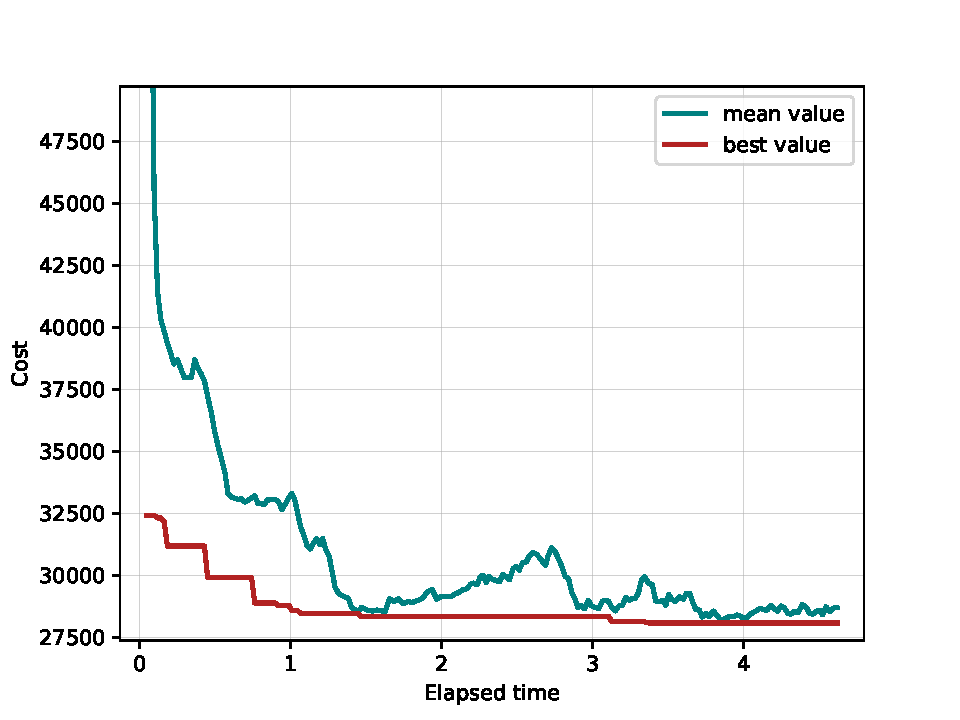
\includegraphics[width=.8\linewidth]{img/convergence.pdf}
    \caption{Typical convergence graph of tour29.csv}
    \label{fig:convergence}
\end{figure}

% convergence graph + explain
% 
Figure~\ref{fig:variations} shows the histograms that are obtained when running the problem 1000 times with the GA:
\begin{figure}[H]
    \begin{subfigure}{0.55\linewidth}
      \centering
      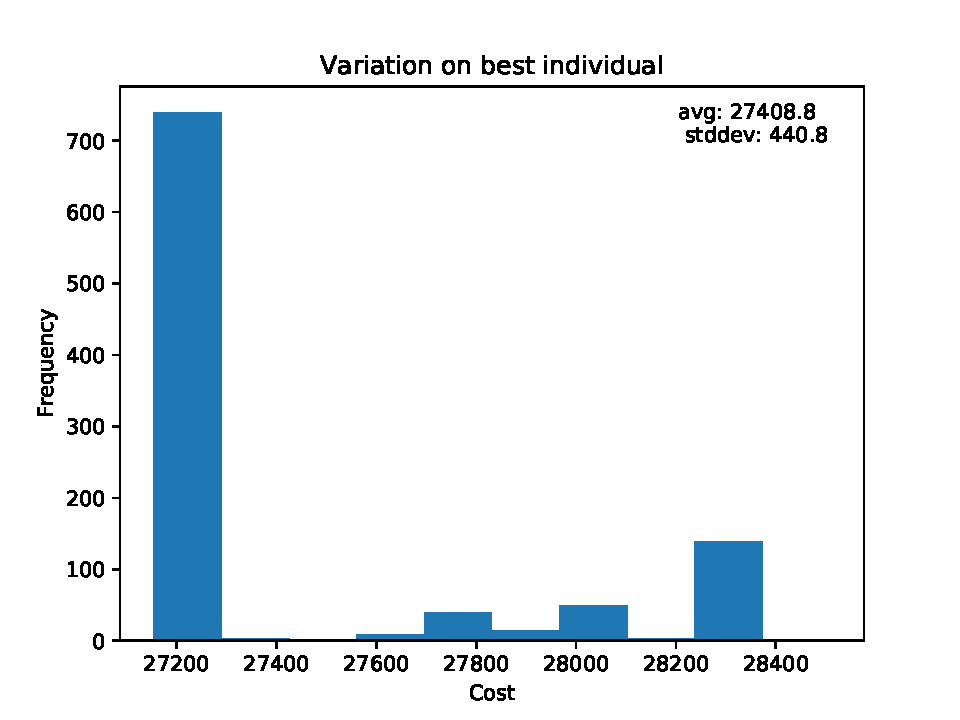
\includegraphics[width=\linewidth]{img/variationbest.pdf}
      \caption{variation on the best individual}
      \label{fig:variationbest}
    \end{subfigure}
    \begin{subfigure}{0.5\linewidth}
      \centering
      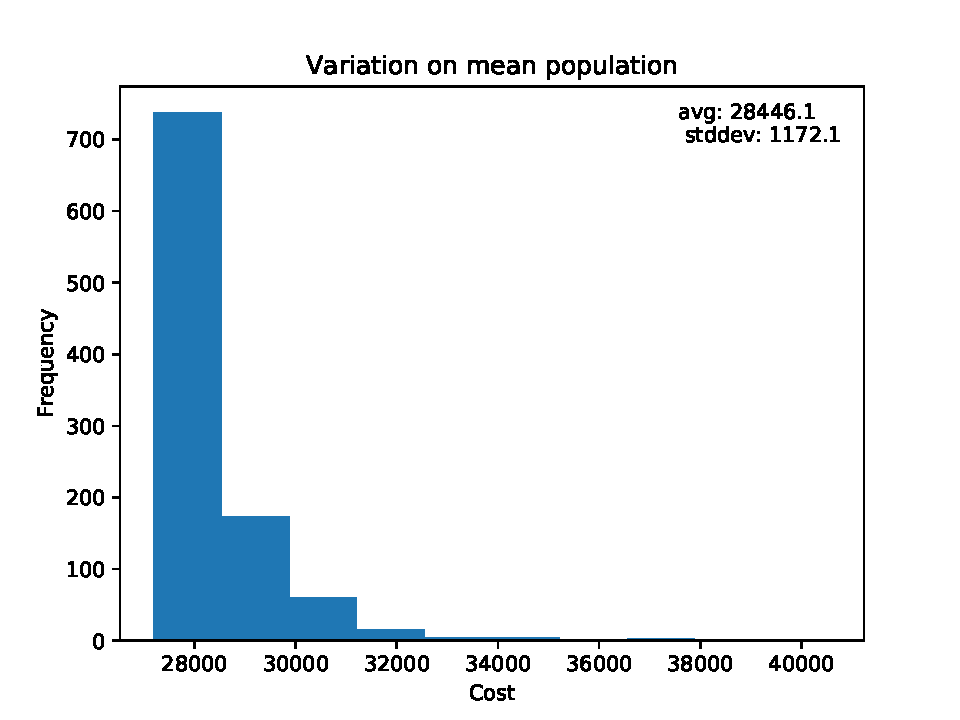
\includegraphics[width=\linewidth]{img/variationmean2.pdf      }
      \caption{variation on the mean individual}
      \label{fig:variationmean}
    \end{subfigure}
    \caption{Histograms that shows the variation on the best individual and mean individual when the problem is run 1000 times}
    \label{fig:variations}
  \end{figure}


\subsection{tour100.csv}

\ReplaceMe{Run your algorithm on this benchmark problem (with the 5 minute time limit from the Reporter). Include a typical convergence graph, by plotting the mean and best objective values in function of the time (for example based on the output of the Reporter class). 

What is the best tour length you found in each case? 

Interpret your results. How do you rate the performance of your algorithm (time, memory, speed of convergence, diversity of population, quality of the best solution, etc)? Is your solution close to the optimal one?}

\subsection{tour194.csv}

\ReplaceMe{Run your algorithm on this benchmark problem (with the 5 minute time limit from the Reporter). Include a typical convergence graph, by plotting the mean and best objective values in function of the time (for example based on the output of the Reporter class). 

What is the best tour length you found? 

Interpret your results. How do you rate the performance of your algorithm (time, memory, speed of convergence, diversity of population, quality of the best solution, etc)? Is your solution close to the optimal one?}

\subsection{tour929.csv}

\ReplaceMe{Run your algorithm on this benchmark problem (with the 5 minute time limit from the Reporter). Include a typical convergence graph, by plotting the mean and best objective values in function of the time (for example based on the output of the Reporter class). 

What is the best tour length you found? 

Interpret your results. How do you rate the performance of your algorithm (time, memory, speed of convergence, diversity of population, quality of the best solution, etc)? Is your solution close to the optimal one? 

Did your algorithm converge before the time limit? How many iterations did you perform?}



\section{Critical reflection}

\RemoveMe{\textbf{Goal:} Based on this section, we will evaluate your understanding and insight into the main strengths and weaknesses of your evolutionary algorithms.}

% \ReplaceMe{Describe the main lessons learned from this project. What do you think are the main strong points of evolutionary algorithms in general? Did you apply these strengths in this project? What are the main weaknesses of evolutionary algorithms and of your implementation in particular? Do you think these can be avoided or mitigated? How? Do you believe evolutionary algorithms are appropriate for this problem? Why (not)? What surprised you and why? What did you learn from this project?}
The main strengths of a GA is in my opinion that it can be used in various representations and thus problems. It can come up relatively fast with good solutions and the basic concept is easy to understand. 
I think the main weakness of a GA is the tuning of the different parameters. There are a lot of parameters to be considered (k in k-tournament, $\alpha$ for mutation, $\lambda$ for population size, $\mu$ for amount of offspring, \ldots). It is time-consuming and sometimes difficult to find out what the best values for these parameters are. One can try to implement self-adaptivity, where the different parameters adapt with every new generation. But there is no 'one size fits all' solution and self-adaptivity is still subject of many studies today.

% parallisern van bewerkingen op arrays zou dingen sneller maken


% \section{Other comments} \label{sec_other}

% \ReplaceMe{In case you think there is something important to discuss that is not covered by the previous sections, you can do it here. }

\end{document}
